% !TeX root = main.tex
% !TeX spellcheck = de_DE

\begin{sheet}
    \begin{problem}[title={Eine interessante Permutation}]
        In unserem FFT-Algorithmus haben wir im Beispiel $n=8$ mit Zahlen $a_0,a_1,\ldots,a_7$ in dieser Reihenfolge begonnen, aber am Ende den fourier-transformierten Vektor in der Reihenfolge $\hat{a}_0, \hat{a}_4, \hat{a}_2, \hat{a}_6, \hat{a}_1,\hat{a}_5, \hat{a}_3, \hat{a}_7$ erhalten.

        Beschreibe die Permutation $\sigma:\set{0,1,\ldots,n-1} \to \set{0,1,\ldots,n-1}$, die dadurch bestimmt ist, dass $\hat{a}_{\sigma(0)}, \hat{a}_{\sigma(1)}, \hat{a}_{\sigma(2)}, \ldots$ genau die Reihenfolge ist, in der der fourier-transformierte Vektor ausgegeben wird.
    \end{problem}

    \begin{problem}[title={FFT ist numerisch stabil}]
        Zeige, dass im Cooley-Tukey-Algorithmus $O(\log(n))$ Nachkommastellen an Genauigkeit verloren gehen:

        Es sei $n=2^\ell$ eine Zweierpotenz, $(a_0,\ldots,a_{n-1})\in\IC^n$ der Vektor, den wir fourier-transformieren wollen und $(b_0, \ldots, b_{n-1})\in\IC^n$ eine Näherung an $a$ mit $\abs{a_j-b_j} < 2^{-m}$. OBdA nehmen wir $\abs{a_j}, \abs{b_j} < 1$ an.

        \begin{subproblem}
            Zeige, dass für die fourier-transformierten Vektoren $(\hat{a}_0,\ldots,\hat{a}_{n-1})$ bzw. $(\hat{b}_0,\ldots,\hat{b}_{n-1})$ gilt:
            \[\abs{\hat{a}_j - \hat{b}_j} < 2^{-m+c\log(n)}\]
            mit einer Konstanten $c\geq 1$, d.h.\ pro Rekursionsstufe gehen $c$ viele Bits an Genauigkeit verloren.
        \end{subproblem}
        \begin{subproblem}
            Natürlich hängt das nicht von der Wahl der Basis $2$ und ist genauso wahr bezüglich jeder anderen Basis $g$.
        \end{subproblem}
        \begin{subproblem}
            Zeige, dass analoges gilt, wenn die Fouriertransformation von $b$ nicht mit den exakten Einheitswurzeln $\zeta_n^0,\zeta_n^1,\ldots$ ausgerechnet wird, sondern stattdessen mit Näherungen $z_j \approx \zeta_n^j$ gerechnet wird.

            Hinweis: Die Näherungen $z_j$ können bessere Näherungen sein, als die $b_j$ es sind.
        \end{subproblem}
        \begin{subproblem}
            Zeige, dass das alles genauso auch für die inverse FFT gilt.
        \end{subproblem}
    \end{problem}

    \begin{problem}
        Es sei $n=2^\ell$ eine Zweierpotenz und $m\in\IN$ beliebig. Finde einen Algorithmus, um $\zeta_n:=e^{2\pi i/n}$ auf $m$ Nachkommastellen genau zu bestimmen. Zeige, dass man mit $O(m\log(n))$ elementaren Operationen mit komplexen Zahlen auskommen kann?

        \smallskip
        Hinweis 1: Um von $\ell$ zu $\ell+1$ zu kommen, muss man eine (bestimmte von den zwei) Quadratwurzel(n) einer komplexen Zahl berechnen.

        Hinweis 2: Quadratwurzeln rechnet man mit Newton-Iteration aus. Starre so lange auf Abbildung~\ref{fig:fft:approximation_zeta_8}, bis dir klar wird, wie man das macht.

        \begin{figure}[ht]
            \centering
            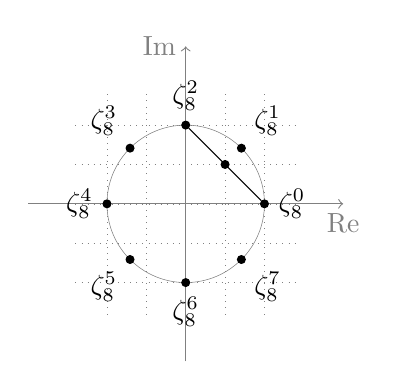
\begin{tikzpicture}[
                dot/.style={draw,fill,circle,inner sep=1pt}
            ]
                \draw[step=0.5,gray,very thin,dotted] (-1.4,-1.4) grid (1.4,1.4);

                \draw[->,gray] (-2,0) -- (2,0) node[below] {Re};
                \draw[->,gray] (0,-2) -- (0,2) node[left] {Im};

                \draw[help lines] (0,0) circle (1);

                \foreach \i in {0,...,7} {
                    \node[dot, label={\i*360/8:$\zeta_8^{\i}$}] (zeta\i) at (\i*360/8:1) {};
                }

                \draw[-,thin] (zeta0) -- (zeta2);
                \node[dot] (zeta1approx) at (0.5,0.5) {};
            \end{tikzpicture}
            \caption{Eine Approximation an $\zeta_8$ ausgehend von $\zeta_4$}
            \label{fig:fft:approximation_zeta_8}
        \end{figure}
    \end{problem}

    \begin{problem}[title={Schönhage-Strassen I}]
        \begin{subproblem}
            Folgere, dass man mit $O(\log(n))$ Bits Genauigkeit rechnen muss, um ganze Zahlen mit $n$ Bits mittels komplexer FFT zu multiplizieren.
        \end{subproblem}
        \begin{subproblem}
            Folgere daraus, dass man ganze Zahlen in $O(n\log(n)^3)$ elementaren Operationen multiplizieren kann.
        \end{subproblem}
        \begin{subproblem}
            Zeige, dass es auch in $O(n\log(n)^2)$ geht, indem statt in Basis $g=2$ in einer größeren Basis $G$ gerechnet wird.
        \end{subproblem}
        \begin{subproblem}
            Folgere daraus wiederum per Induktion, dass es auch in
            \[O(n\cdot\log(n)\cdot \log(\log(n)) \cdots (\log^k(n))^2)\]
            geht.
        \end{subproblem}
    \end{problem}
\end{sheet}